% start the document

% specify the document layout and font size
\documentclass[preprint,12pt]{elsarticle}
\usepackage[margin=1.5cm,includefoot]{geometry}
\usepackage{setspace}

% uploading packages
\usepackage{graphicx}
\usepackage{amssymb}
\usepackage{gensymb}
\usepackage{lineno}
\usepackage{mathtools}
\usepackage[colorlinks]{hyperref}
\usepackage[nameinlink]{cleveref} %needs to appear after hyperref, https://tex.stackexchange.com/questions/396728/my-equations-referencing-not-working
\Crefname{figure}{Figure}{Figures} %needs to appear after hyperref and cleveref
\newcommand\crefrangeconjunction{--} % modify the reference style
\usepackage{mathrsfs}
\usepackage{url}
\usepackage{enumitem}
\usepackage{tabulary}
\usepackage{multirow}
\graphicspath{{figures/}} %Setting the graphicspath
% ---------to deal with the double quotes----------- 
\usepackage [english]{babel}
\usepackage [autostyle, english = american]{csquotes}
\MakeOuterQuote{"}
%alternatively can use `` '' format for double quotes

\usepackage[shortcuts,abbreviations]{glossaries-extra}
\glssetcategoryattribute{abbreviation}{indexonlyfirst}{true}
\glssetcategoryattribute{abbreviation}{nohyper}{true}
\makeglossaries

\newabbreviation{5dof}{5DOF}{five degree-of-freedom}
\newabbreviation{ebsd}{EBSD}{electron backscatter diffraction}
\newabbreviation[longplural={grain boundaries}]{gb}{GB}{grain boundary}
\newabbreviation{mfc}{MFC}{mass flow controller}
\newabbreviation{sem}{SEM}{scanning electron microscope}
\newabbreviation{fea}{FEA}{finite element analysis}
\newabbreviation{bcs}{BCs}{boundary conditions}
\newabbreviation[longplural={triple junctions}]{tj}{TJ}{triple junction}
\newabbreviation{gpr}{GPR}{Gaussian process regression}
\newabbreviation{ann}{ANN}{artificial neural network}
\newabbreviation{nn}{NN}{nearest neighbor}
\newabbreviation{rmse}{RMSE}{root mean square error}
\newabbreviation{mae}{MAE}{mean absolute error}
\newabbreviation{brk}{BRK}{Bulatov Reed Kumar}
\newabbreviation{gbed}{GBED}{grain boundary energy distribution}
\newabbreviation{mfz}{MFZ}{misorientation fundamental zone}
\newabbreviation{bp}{BP}{boundary plane}
\newabbreviation{knn}{k-NN}{k-nearest neighbor}
\newabbreviation{gbe}{GBE}{grain boundary energy}
\newabbreviation{gbo}{GBO}{grain boundary octonion}
\newabbreviation{oslerp}{oSLERP}{octonion Spherical Linear Interpolation}
\newabbreviation{loocv}{LOOCV}{leave-one-out cross validation}
\newabbreviation{kfcv}{kFCV}{k-fold cross validation}
\newabbreviation{seo}{SEO}{symmetrically equivalent octonion}
\newabbreviation{fex}{FEX}{file exchange}
\newabbreviation{idw}{IDW}{inverse-distance weighting}
\newabbreviation{fic}{FIC}{fully independent conditional}
\newabbreviation{svd}{SVD}{singular value decomposition}
% example abbreviations
% \newabbreviation{seo}{SEO}{symmetrically equivalent octonions}
%\newabbreviation[longplural={grain boundaries}]{gb}{GB}{grain boundary}

%example usage: \gls{gpr}
%example usage: \Gls{gpr} (capitalize first letter, only meaningful for first usage)
% \glspl{seo} --> symmetrically equivalent octonions OR SEOs
%^^^^^^^^^^^^^^^^^^^^^^^^^^^^^^^^^^^^^^^^^^^^^^^^^^^


%\title{Grain Boundary Octonion Meshing and Interpolation}
\title{Five degree-of-freedom property interpolation of arbitrary grain boundaries in a closed-octonion mesh}
\author{Sterling G. Baird}
\author{Oliver K. Johnson}
\date{August 2020}

% Double Spacing
\doublespacing
\begin{document}

\begin{abstract}
    The closed-octonion interpolation framework offers an advantage over other five-degree-of-freedom based property interpolation methods because it's defined as a closed mesh in a Riemannian manifold. One can triangulate a mesh using standard routines (e.g. quickhull, qhull.org) and interpolate using barycentric coordinates or machine learning methods such as Gaussian Process Regression. Euclidean and arc length distances take on meaning in this framework and are trivial computations compared with other distance metrics, thereby addressing a limitation in previous work. The ability to use significantly more input data lends itself to lower interpolation error and is demonstrated by grain boundary energy interpolation results for a non-smooth validation function (Bulatov, Reed, Kumar) and simulated bi-crystal datasets from the literature for Ni and Fe. Four interpolation methods built on this framework --- barycentric interpolation, Gaussian Process Regression or Kriging, inverse-distance weighting, nearest neighbor interpolation --- are presented and compared against a constant, average model (RMSE = 0.013 $J/m^2$), resulting in RMSE values of 0.063, 0.056, 0.068, and 0.082 $J/m^2$, respectively, for 50,000 randomly input sampled bicrystals and evaluated for 10,000 randomly sampled output bicrystals. A vectorized, parallelized, MATLAB implementation is made available (github.com/sgbaird-5dof/interp) with similar input/output structure of built-in MATLAB interpolation functions (e.g. \textit{interpn}) and placeholders for custom interpolation schemes. The closed-octonion framework offers a great advantage in estimating property values for arbitrary grain boundaries based on experimental or simulated data and modeling surrogates of computationally expensive 5DOF functions and simulations.
\end{abstract}

\maketitle

\section{Introduction} \label{sec:intro}

Others have developed tools or generated models to describe a \gls{5dof} property based on experimental or simulated data. The Rohrer group used binning and gradient descent to solve for \gls{5dof} \gls{gbed} in nickel \cite{liRelativeGrainBoundary2009}, yttria \cite{dillonCharacterizationGrainboundaryCharacter2009}, and copper \cite{randleFiveparameterGrainBoundary2008} based on experimentally characterized 3D microstructures. A non-discretizing approach was recently introduced by Rohrer's group (2019) that utilizes regularization imposed on triple junction equilibrium equations, the Locally Optimal Block Preconditioned Conjugate Gradient method, and \gls{knn} distances \cite{shenDeterminingGrainBoundary2019}. In this approach, 60,000 \glspl{tj} and a custom, non-smooth validation function are used to obtain \gls{gbe} \gls{rmse} values of approximately 0.01 and 0.03 $mJ/m^2$ for \gls{gbe} values less than 0.9 $J/m^2$ and greater than 0.9 $J/m^2$, respectively. Restrepo et. al. uses an \gls{ann} and approximately 17,000 Kim Fe bicrystal simulations \cite{kimIdentificationSchemeGrain2011} as training data to achieve \gls{mae} errors of approximately 50 $mJ/m^2$ and 90 $mJ/m^2$ in the best fitted \glspl{ann} for randomly selected and special \glspl{gb}, respectively \cite{echeverrirestrepoUsingArtificialNeural2014}. Recently (2019), De Graef and Holm's groups at CMU reported and tested a new \gls{gb} representation, which they term \glspl{gbo} \cite{francisGeodesicOctonionMetric2019,chesserLearningGrainBoundary2020}.

The \gls{gbo} distance metric offers an advantage over other metrics in that it "correctly determines the angular distances between \glspl{gb} with a common normal or misorientation" and "closely approximates the geodesic metric on $SO(3) \times SO(3)$ \textit{for all grain boundary pairs} while maintaining the ability to be analytically minimized with respect to the $U(1)$ symmetry" \cite{francisGeodesicOctonionMetric2019}. A derivation and examples of \gls{oslerp} is given which produces smooth, minimum distance paths through \gls{gb} character space between two arbitrary \glspl{gb}. Laplacian kernel regression (a type of inverse distance weighting) involving scaled pairwise distance matrices were later used to obtain a model for describing properties of arbitrary \glspl{gb} \cite{chesserLearningGrainBoundary2020}. Using \gls{kfcv} with $k=10$ for the 388 Olmsted Ni \glspl{gb}, an \gls{rmse} of 0.0977 $J/m^2$ is obtained using an optimized scaling parameter. Due to computation time of pairwise distance matrices, this approach is limited to datasets with several thousand or fewer \glspl{gb} \cite{chesserLearningGrainBoundary2020}.

The closed-octonion interpolation framework presented in this work offers an advantage over other methods because it's defined as a closed mesh in a Riemannian manifold. This is evidenced by the ability to triangulate a mesh using standard routines (e.g. quickhull \cite{barberQuickhullAlgorithmConvex1996}) and interpolate using barycentric coordinates or machine learning methods such as \gls{gpr}. Extending previous work on \glspl{gbo} \cite{francisGeodesicOctonionMetric2019,chesserLearningGrainBoundary2020}, we obtain a closed mesh by obtaining a set of octonions minimized with respect to Euclidean distance and an arbitrary reference octonion after considering all \glspl{seo}. Because \glspl{gbo} are guaranteed to reside on the surface of a hypersphere \cite{francisGeodesicOctonionMetric2019} (a type of Riemannian manifold) a closed mesh is thus formed which locally resembles Euclidean space (\ref{sec:methods}).

Because Euclidean and arc length distances take on meaning in this framework, distance computations are trivial compared with other metrics (even the original octonion distance given in \cite{francisGeodesicOctonionMetric2019}). For example, a 50,000 x 50,000 pairwise-distance matrix can be computed in minutes -- something that was computationally unrealistic before and a limitation of previous work. Compared to the original octonion metric, this represents an improvement in computational speed by about three to four orders of magnitude. This is due to the fact that symmetrically equivalent \glspl{gb} only need to be considered once per \gls{gb}, $O(N_p^2L)$, rather than once per distance calculation per \glspl{gb} in a \gls{gb}-pair, $O(N_p^4L^2)$, where $N_p$ is the symmetry cardinality ($N_p=24$ for $m\Bar{3}m$ FCC point group) and $L$ is the number of \glspl{gb}. % $O(N^2L)$ (this work) vs. $O(N^4L^2$ (octonion paper)

The ability to use significantly more input data lends itself to lower interpolation error and is demonstrated by \gls{gbe} interpolation results for a non-smooth validation function (\gls{brk} \cite{bulatovGrainBoundaryEnergy2014}) and simulated bi-crystal datasets from the literature (388 Olmsted Ni \cite{olmstedSurveyComputedGrain2009} and 50,000 Kim Fe \cite{kimIdentificationSchemeGrain2011} bicrystals). Four interpolation methods built on this framework --- barycentric (\ref{sec:methods:bary}), \gls{gpr} or Kriging (\ref{sec:methods:gpr}), \gls{idw} (\ref{sec:methods:idw}), \gls{nn} (\ref{sec:methods:nn}) --- are presented and compared against a constant, average model (\ref{sec:resultsDiscussion}). For the convenience of the reader, a vectorized, parallelized, MATLAB implementation is made available (github.com/sgbaird-5dof/interp) with similar input/output structure of built-in MATLAB interpolation functions (e.g. interpn) and placeholders for custom interpolation schemes. Input and prediction points (misorientation/\gls{bp} normal pairs or octonions) and property values are supplied, and interpolated/predicted values are output.

The closed-octonion framework offers a great advantage in estimating property values for arbitrary \glspl{gb} based on experimental or simulated data such as energy, mobility, and diffusivity. The framework can also enable surrogate modeling of computationally expensive 5DOF functions and simulations such as in evaluation of the \gls{brk} function or anisotropic grain growth simulations.

\section{Results and Discussion} \label{sec:resultsDiscussion}

\begin{enumerate}

    \item A parity plot is provided for the four interpolation methods considered in this work --- barycentric interpolation (\ref{sec:methods:bary}), Gaussian Process Regression or Kriging (\ref{sec:methods:gpr}), inverse-distance weighting (\ref{sec:methods:idw}), nearest neighbor interpolation (\ref{sec:methods:nn}) --- for 50,000 randomly sampled (\ref{sec:methods:rand}) input \glspl{gb} and 10,000 randomly sampled prediction \glspl{gb} (Figure \ref{fig:brkparity50000}).

    \begin{enumerate}
        \item There is a concentration of high \glspl{gbe} near 1.2 $J/m^2$, which is in the same region as the average \gls{gbe} obtained via many random \gls{gb} samples. This makes it difficult to compare error metrics with other models where an even sampling across \glspl{gbe} is obtained. To aid in objective interpretation, the errors can be compared to that obtained via a constant, average model (approximately 1.16 $J/m^2$) resulting in \gls{rmse} and \gls{mae} values of approximately 0.130 and 0.097 $J/m^2$.
        \item barycentric interpolation both underestimates and overestimates
        \item \Gls{gpr} has the lowest error of the four interpolation methods.
        \item \Gls{gpr} tends to overestimate rather than underestimate \gls{gbe}.
        \item Barycentric interpolation is fast once the triangulation is computed (i.e. still fast even if responses change, but needs to be recomputed if input data, i.e. predictors, change). \Gls{gpr} is fast and has lower error compared to barycentric interpolation; however, the entire process has to be rerun (in current implementation) if the responses or the predictors change.
        \item \Gls{idw} systematically overestimates and underestimates low and high \glspl{gbe}, respectively, similar to what's described in \cite{chesserLearningGrainBoundary2020}. Based on the similarity of approaches between \cite{chesserLearningGrainBoundary2020} and this work's \gls{idw}, we surmise that \gls{idw} is not the most appropriate interpolation method for \gls{gbe}; however, it is unclear how \gls{idw} would perform for other properties.
        \item \Gls{nn} has the highest error of the four interpolation methods, and has a fairly even spread of underestimation and overestimation regardless of the energy.
    \end{enumerate}
    
    \item A histogram of \gls{nn} octonion distances is provided for the mesh with 50,000 octonions (Figure \ref{fig:nndist}).
    \begin{enumerate}
        \item This exhibits symmetric, normal distribution behavior with a slight skew towards lower distances.
        \item The mean and standard deviation of this mesh are 2.8651 and 0.69452 degrees, respectively.
    \end{enumerate}
    
\end{enumerate}

\begin{figure}
    \centering
    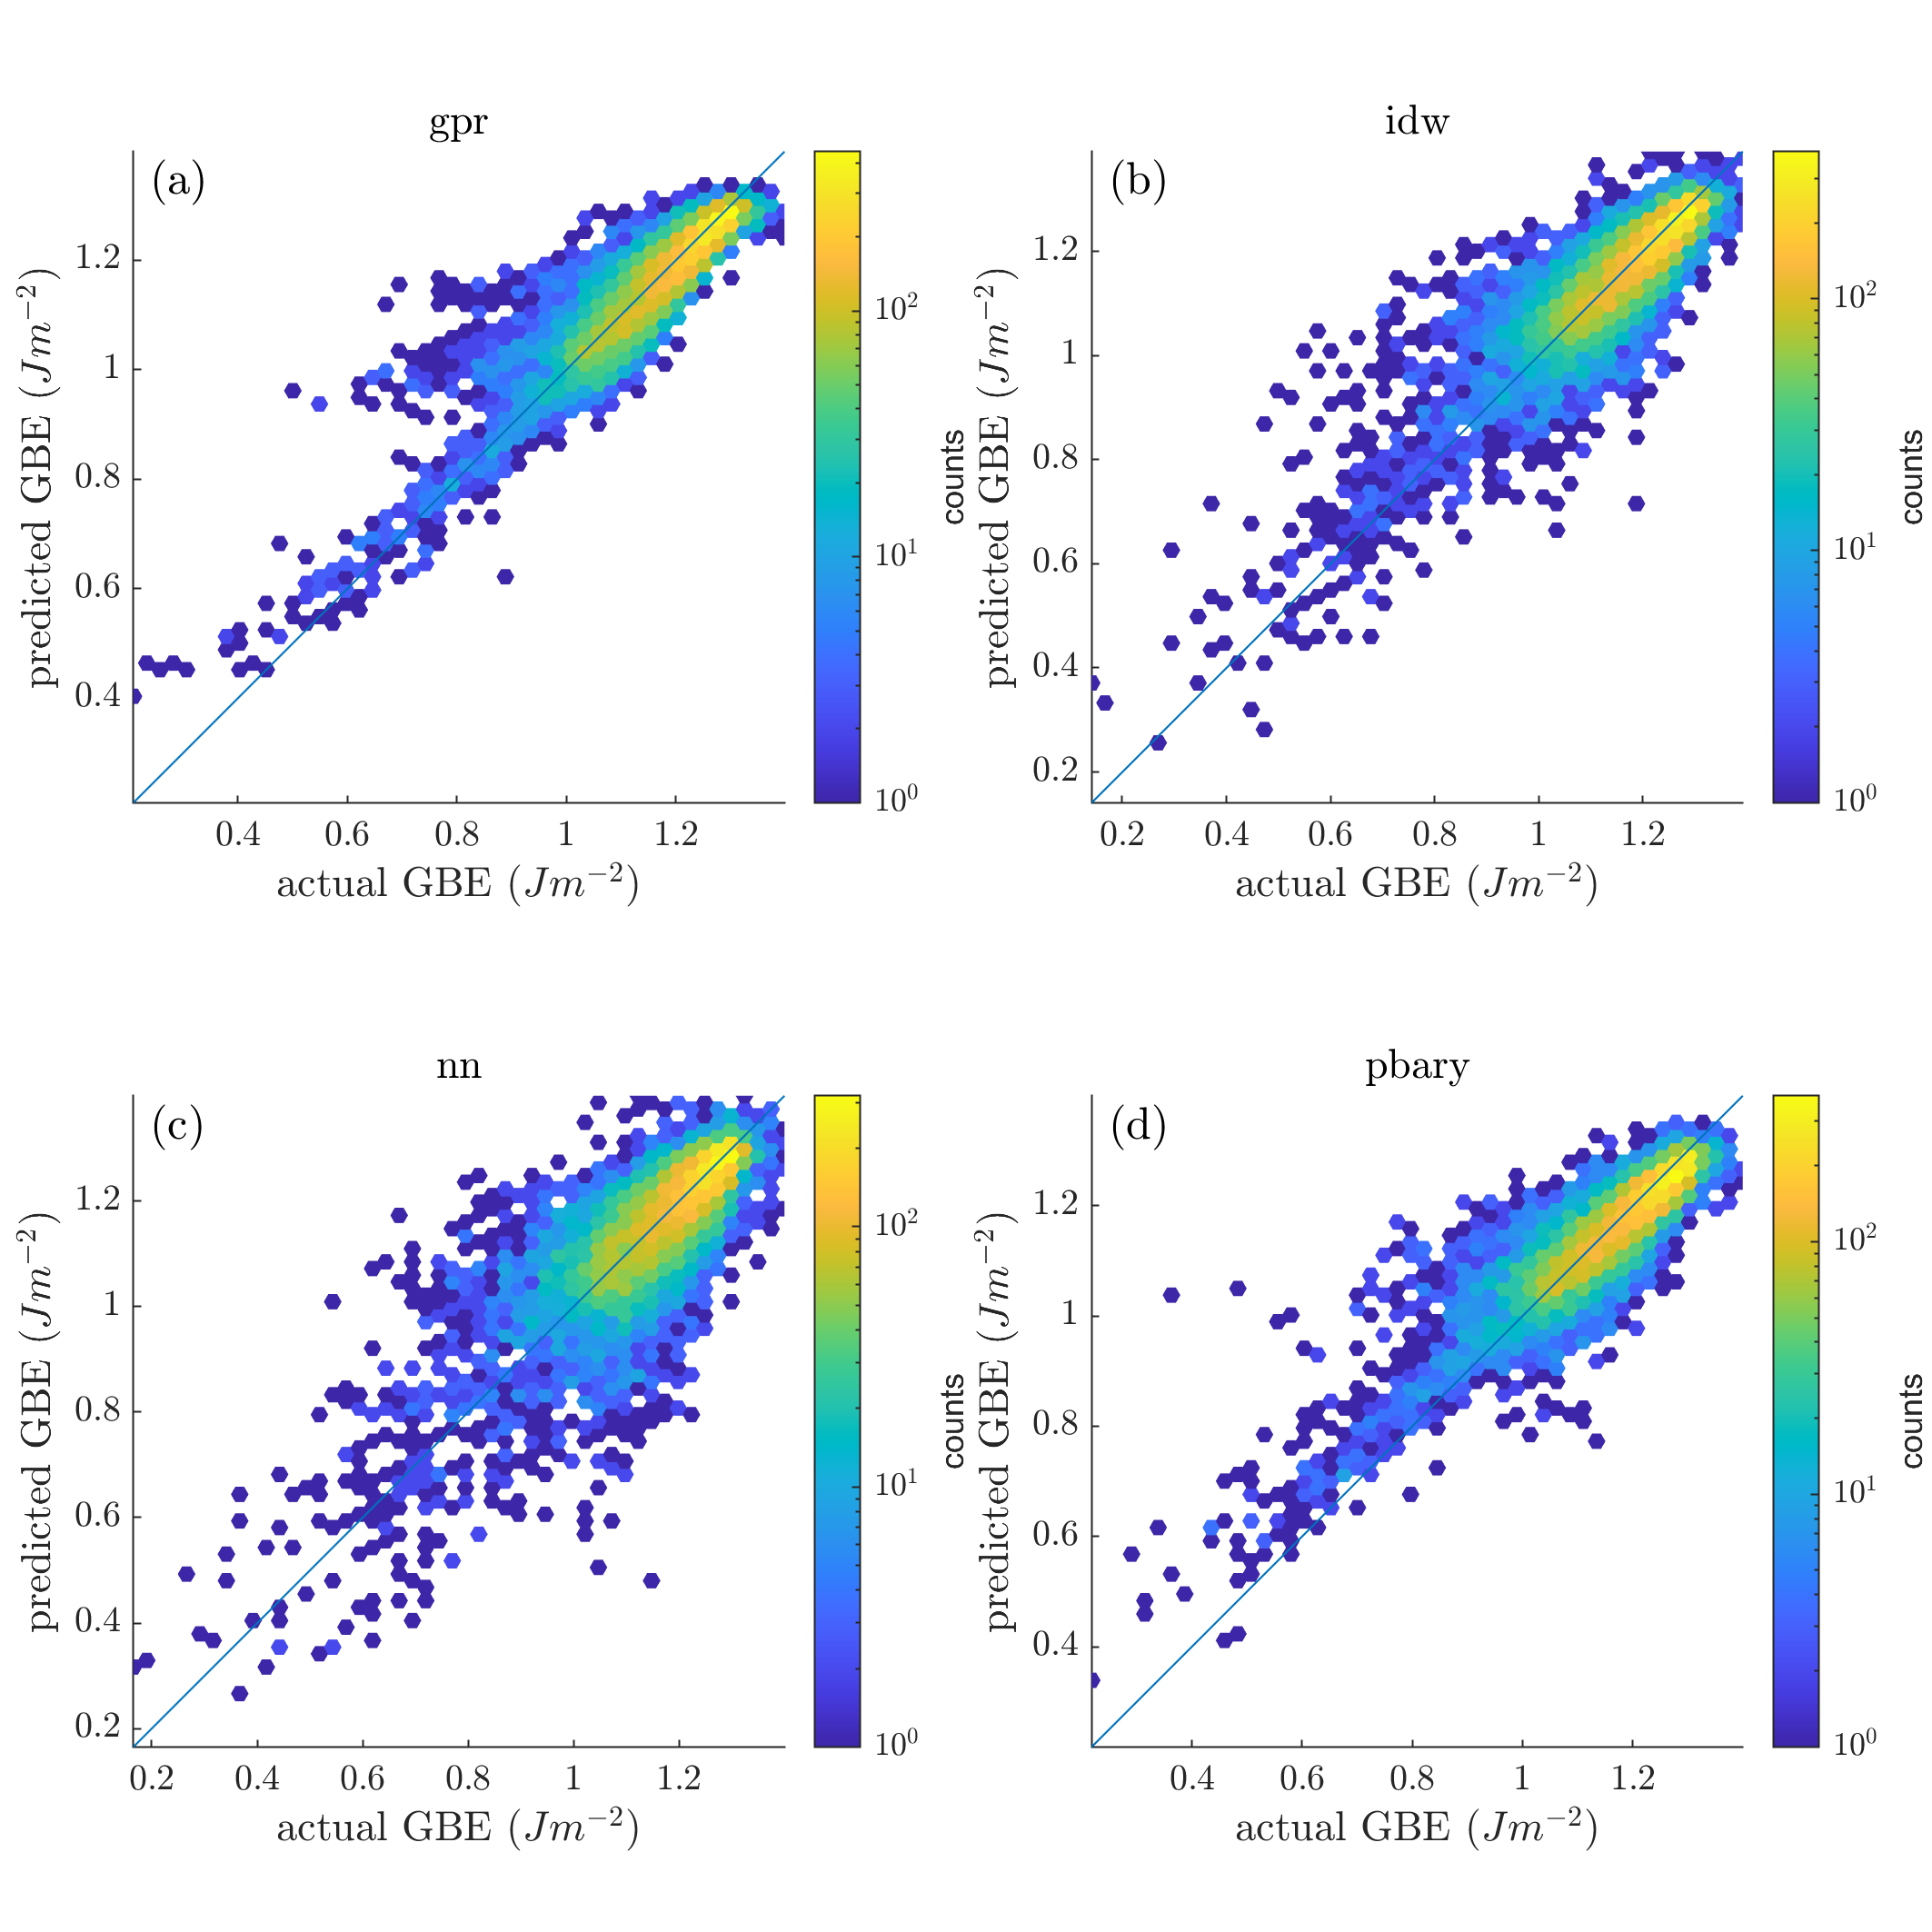
\includegraphics{brkparity50000.png}
    \caption{Parity plot for 50000 mesh and 10000 prediction octonions formed via pairs of a random cubochorically sampled quaternion and a spherically sampled random boundary plane normal. Interpolation via \acrlong{gpr} (a), \acrlong{idw} (b), \acrlong{nn} (c), and barycentric coordinates (d). Property values sampled via \acrlong{brk} \acrlong{gbe} function.}
    \label{fig:brkparity50000}
\end{figure}

\begin{figure}
    \centering
    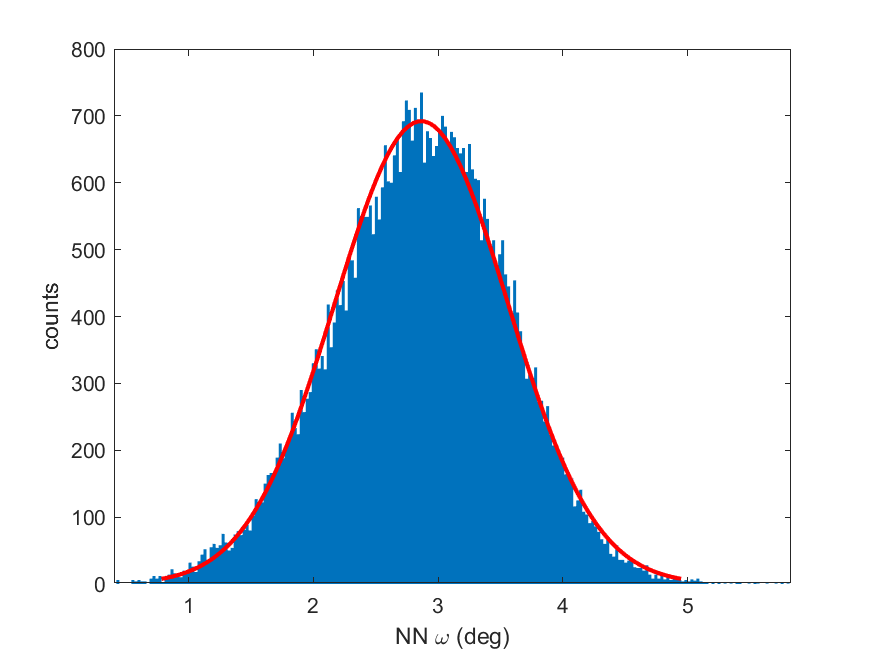
\includegraphics{disthist50000.png}
    \caption{Histogram of \acrfull{nn} octonion distances ($\omega$) for 50,000 octonions formed via pairs of a random, cubochorically sampled quaternion and a random \acrfull{bp} unit vector normal.}
    \label{fig:nndist}
\end{figure}

\begin{figure}
    \centering
    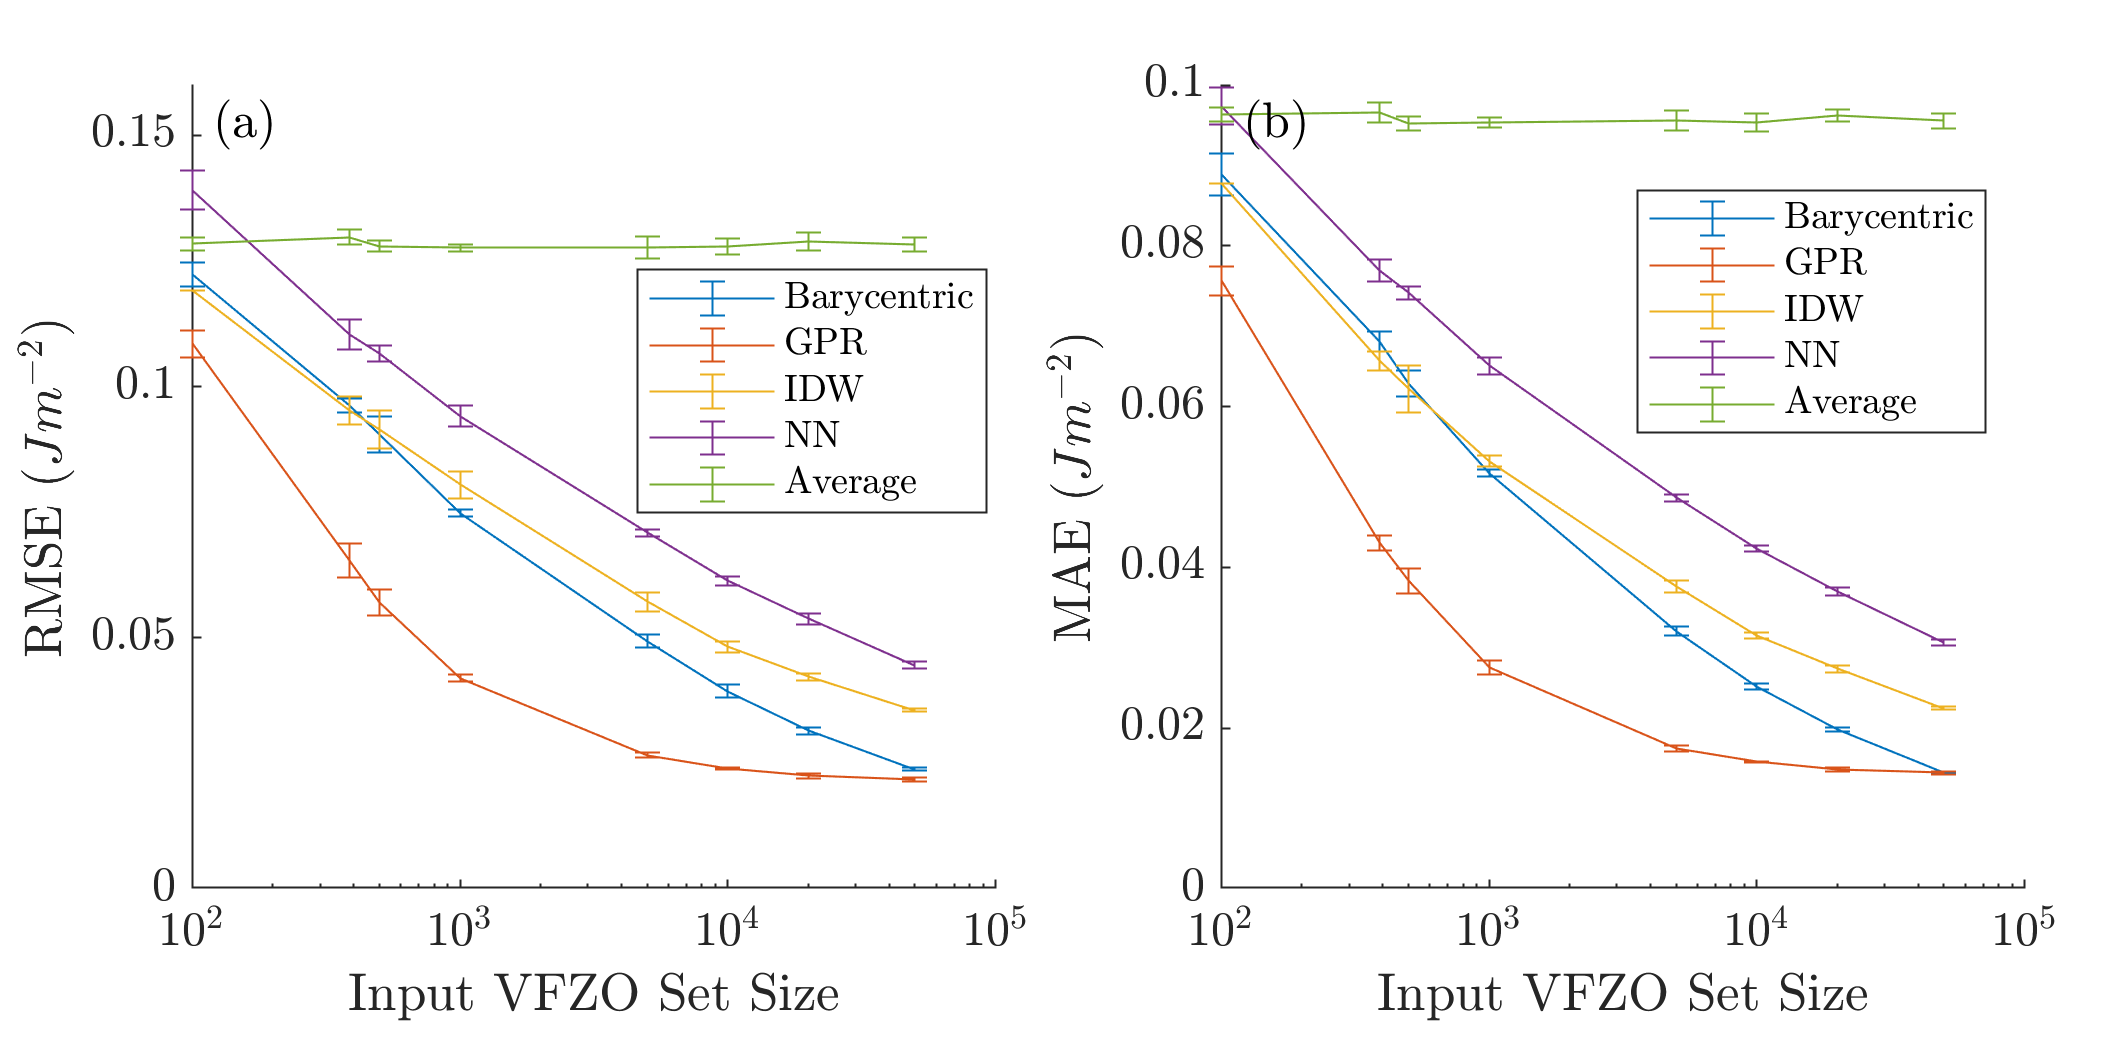
\includegraphics{brkerror.png}
    \caption{Average \acrlong{rmse} and average \acrlong{mae} vs. number of mesh points for barycentric (blue), \acrlong{gpr} (\acrshort{gpr}) (orange), \acrlong{idw} (\acrshort{idw}) (yellow), and \acrlong{nn} (\acrshort{nn}) (purple) interpolation for 10 random runs with different mesh and prediction points. Standard deviations of the 10 runs are also included. Compare with approximately 0.13 $J/m^2$ and 0.95 $J/m^2$ \acrshort{rmse} and \acrshort{mae}, respectively, for a constant model using the average of the mesh properties (approximately 1.16 $J/m^2$).}
    \label{fig:brkerror}
\end{figure}

\begin{figure}
    \centering
    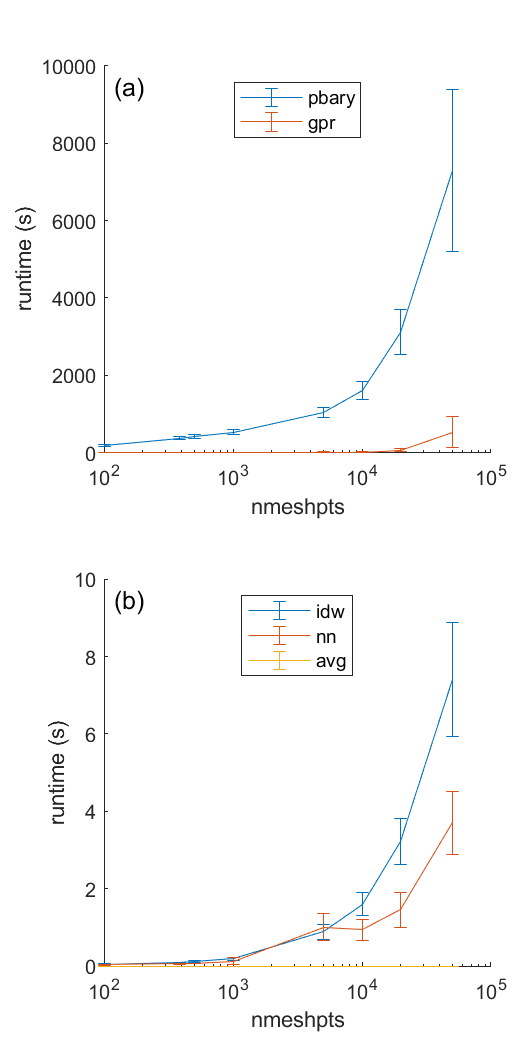
\includegraphics{runtime.png}
    \caption{Runtime (s) vs. number of mesh points for barycentric (blue), \acrlong{gpr} (\acrshort{gpr}) (orange), \acrlong{idw} (\acrshort{idw}) (yellow), and \acrlong{nn} (\acrshort{nn}) (purple) interpolation using 24 cores. Because \acrshort{gpr}, \acrshort{idw}, and \acrshort{nn} method defaults are single-threaded, the number of cores only significantly affects the runtime of barycentric interpolation.}
    \label{fig:runtime}
\end{figure}

% \begin{figure}
%     \centering
%     \includegraphics{}
%     \caption{Parity plot for 388 mesh and 10000 prediction octonions formed via pairs of a random cubochorically sampled quaternion and a spherically sampled random boundary plane normal. Interpolation via \acrlong{gpr} (a), \acrlong{idw} (b), \acrlong{nn} (c), and barycentric coordinates (d). Property values sampled via \acrlong{brk} \acrlong{gbe} function.}
%     \label{fig:brkparity388}
% \end{figure}

% \begin{enumerate}
    % \item parity plots
    % \begin{enumerate}
    %     \item 388, 10,000, and 50,000 mesh points
    %     \item tile1 - barycentric
    %     \item tile2 - \gls{gpr}
    %     \item tile3 - inverse-distance weighting
    %     \item tile4 - pure \gls{nn} interpolation
    % \end{enumerate}

    % \item \Gls{rmse} vs. number mesh points for barycentric interpolation (black), \gls{gpr}, and pure \gls{nn} interpolation (red). Range from 1e2 to 1e5 mesh points

    % \item histograms of \gls{nn} and next \gls{nn} distances (arc length) for mesh
    % \begin{figure}
    %     \centering
    %     \includegraphics{}
    %     \caption{histograms of \acrfull{nn} (red) and next \acrlong{nn} (black) arc lengths for meshes of 388 (a), 10,000 (b), and 50,000 (c) octonions formed via pairs of random, cubochorically sampled quaternions.}
    %     \label{fig:nndist}
    % \end{figure}

%     \item timing and efficiency
%     \begin{enumerate}

%     \end{enumerate}
%     \item comparison with Chesser \cite{Chesser2020LearningProperties} (few points, Ni data, both high- and low-symmetry sets). Use 388 Ni bicrystals instead of \gls{brk} function. Barycentric and \gls{gpr}
%     \begin{enumerate}
%         \item table
%         \begin{table}[]
%             \centering
%             \begin{tabular}{c c c c}
%                 \hline
%                  Method & Minimizing Distance & \acrshort{rmse} & \acrshort{mae} \\
%                  \hline
%                  Barycentric & Euclidean Norm & & \\
%                  \acrshort{nn} & Euclidean Norm & & \\
%                  \acrshort{gpr} & Euclidean Norm & & \\
%                  Pairwise-distance & Arc Length & &
%             \end{tabular}
%             \caption{Comparison of \acrfull{rmse} and \acrfull{mae} for closed-mesh barycentric interpolation, closed-mesh \acrfull{nn} interpolation, closed-mesh \acrfull{gpr}, and pairwise-distance inverse weighting for 388 Ni bicrystal simulations with 10-fold cross validation for each method.}
%             \label{tab:chesser-comp}
%         \end{table}
%         \item parity plot
%         \item \gls{5dof} visualizations
%         \begin{figure}
%             \centering
%             \includegraphics{}
%             \caption{\acrfull{gb} energy plotted in the $\Sigma{3}$, $\Sigma{5}$, $\Sigma{7}$, and $\Sigma{11}$ \acrlong{bp} spaces for closed-mesh spherical barycentric (a) and \acrlong{nn} (b) interpolation, closed-mesh \acrlong{gpr} (c), and pairwise-distance inverse weighting using 388 Ni bicrystal simulations.}
%             \label{fig:chesser-5dof}
%         \end{figure}
%         \item 1DOF curves ([100] and [110] symmetric tilt boundaries ?)
%     \end{enumerate}
%     \item comparison with Restrepo \cite{EcheverriRestrepo2014UsingEnergies} (many points, Fe data, both high- and low-symmetry sets). Use simulated Fe data instead of \gls{brk} function. Barycentric and \gls{gpr}
%     \begin{enumerate}
%         \item table
%         \begin{table}[]
%             \centering
%             \begin{tabular}{c c c c}
%                 \hline
%                  Method & Minimizing Distance & \acrshort{rmse} & \acrshort{mae} \\
%                  \hline
%                  Barycentric & Euclidean Norm & & \\
%                  \acrshort{nn} & Euclidean Norm & & \\
%                  \acrshort{gpr} & Euclidean Norm & & \\
%                  \acrshort{ann} & N/A & &
%             \end{tabular}
%             \caption{Comparison of \acrfull{rmse} and \acrfull{mae} for closed-mesh barycentric interpolation, closed-mesh \acrlong{gpr}, and a non-symmetry considering \acrfull{ann} using 50,000 Fe bicrystal simulations.}
%             \label{tab:restrepo-comp}
%         \end{table}
%         \item parity plot
%         \item \gls{5dof} visualizations
%         \begin{figure}
%             \centering
%             \includegraphics{}
%             \caption{\acrfull{gb} energy plotted in the $\Sigma{3}$, $\Sigma{5}$, $\Sigma{7}$, and $\Sigma{11}$ \acrlong{bp} spaces for closed-mesh spherical barycentric (a) and \acrlong{nn} (b) interpolation, closed-mesh \acrlong{gpr} (c), and a non-symmetry considering \acrlong{ann} (d) using 50,000 Fe bicrystal simulations.}
%             \label{fig:restrepo-5dof}
%         \end{figure}
%         \item 1DOF curves ([100] and [110] symmetric tilt boundaries ?)
%     \end{enumerate}
% \end{enumerate}

\section{Methods} \label{sec:methods}

\subsection{Closed-mesh Octonions vs. Original Octonion Metric} \label{sec:methods:closed-mesh}

In the closed-mesh octonion framework, \glspl{seo} are chosen based on minimum Euclidean distance relative to a fixed, arbitrary reference octonion rather than allowing either octonion in a pair to vary in the traditional octonion approach with arc-length distances \cite{francisGeodesicOctonionMetric2019}. We consider all symmetrically equivalent \glspl{gbo} rather than a subset. We also remove a degenerate dimension to 7D Cartesian for barycentric interpolation and employ a further projection to 6D Cartesian for the triangulation. These differences are summarized in Table \ref{tab:closed-mesh-comparison}. By choosing symmetrically equivalent representations of octonions based on Euclidean distance with respect to a fixed octonion, a "closed-mesh" is obtained in the sense that directly computed Euclidean and arc length distances become meaningful and a unique octonion is found within numerical tolerance as long as the reference \gls{gbo} is low-symmetry (very likely based on random sampling and can be verified). This facilitates the use of standard triangulation and interpolation routines rather than needing to rely on pairwise-distance matrices where each distance calculation requires consideration of \glspl{seo}.

% either octonion is allowed to vary to vary for efficiency, whereas in ours, one octonion is held constant. 
%                 \item traditional: use arc length as minimizing metric; ours: use euclidean norm
%                 \item traditional: consider a subset of symmetrically equivalent GBOs; ours: consider all symmetrically equivalent GBOs
%                 \item traditional: always stay in 8D representation; ours: remove degenerate dimension (to 7D) for interpolation and employ projections (to 6D) for triangulation efficiency (for barycentric interpolation)
  
        % \item triangulating a set of octonions using qhull (for barycentric interpolation)
        % \item projections and rotations (projection to hyperplane, singular value decomposition)
        % \item spherical barycentric coordinates \cite{Langer2006SphericalCoordinates}
        % \begin{enumerate}
        %     \item equations
        % \end{enumerate}
        % \item barycentric interpolation
        % \begin{enumerate}
        %     \item equations
        %     \item Determine intersecting facet using facets connected to \gls{nn}s and positivity constraint of planar barycentric coordinates
        %     \item intersecting facet vertices projected onto hyperplane tangent to hypersphere at datapoint
        %     \item containing facet and barycentric coordinates only need to be computed once for each datapoint, can be easily reused
        % \end{enumerate}

    % \item random cubochoric sampling \cite{Singh2016OrientationMethods}
    % \item use of \gls{brk} function \cite{Bulatov2014GrainMetals}
    
    % \item training, validation, and test partitioning \cite{Wang2020MachinePractices} for Kim data set \cite{Kim2011AnDatabase}


\subsection{Barycentric Interpolation} \label{sec:methods:bary}

Barycentric interpolation is commonly used for interpolation within a simplex or other convex polygon. Basic equations of positivity, partition of unity, and linear precision are given in \cite{langerSphericalBarycentricCoordinates2006}, as well as a treatment of linear-precision preserving spherical barycentric coordinates. Because octonion distances are well-approximated by Euclidean distances in a closed-octonion mesh and both distance metrics result in similar error results, only a treatment of Euclidean distances is presented here. However, spherical barycentric coordinates are still included as an option to the MATLAB implementation of this work, \textit{interp5DOF}. For interested readers, a treatment of spherical barycentric coordinates that preserve partition of unity rather than linear-precision is given in \cite{leiNewCoordinateSystem2020}, favoring even subdivision of spherical surfaces rather than interpolation accuracy.

In order to reduce the computationally complexity of computing barycentric coordinates in a high-dimensional space \cite{barberQuickhullAlgorithmConvex1996}, a single degenerate dimension (originally introduced by analytically minimizing $U(1)$ symmetry) is removed. This is done via a \gls{svd} projection, analogous to a Cartesian rotation and translation. Thus, a set of octonions originally represented by 8D Cartesian coordinates are collapsed to a 7D Cartesian representation while preserving both distances and angles among the points \cite{}. To further reduce the "curse of dimensionality" in computing the triangulation, a 7D Cartesian representation of the octonions constrained to lie on the surface of the 6-sphere are first projected onto a hyperplane tangent to the mean of the input points and then rotated/translated again via \gls{svd} to produce a 6D Cartesian representation. This 6D representation is used to compute a triangulation via the built-in MATLAB routine \textit{delaunayn} based on the quickhull algorithm \cite{barberQuickhullAlgorithmConvex1996}, giving facet vertices for the 7D Cartesian hypersphere.

Separate from the mesh triangulation, a new projection of the original octonions to 7D Cartesian coordinates takes place simultaneously for input and prediction points to preserve distances and angles \textit{between each set} as well as \textit{within each set}. Despite having different \glspl{svd}, the 6D Cartesian triangulation holds for either 7D Cartesian representation because the two 7D Cartesian representations are homeomorphic to each other (i.e. distance- and angle-preserving).

Due to the vast number of facets per point of a high-dimensional spherical triangulation and for computational speed, a given prediction point intersection within the input mesh is determined by considering facets connected to up to some number of \glspl{nn} in the mesh (in this work, 10 \glspl{nn}) relative to the prediction point. In cases where an intersecting facet is not found due to high-aspect ratio facets or prediction point falling outside the mesh within a given tolerance, \gls{nn} interpolation and extrapolation are used, respectively, with an identical implementation for interpolation and extrapolation given in \ref{sec:methods:nn}.

Once barycentric coordinates are computed for a prediction point within the input mesh, the interpolated value is found by taking the dot product of the barycentric coordinates and the properties of the corresponding vertices of the intersecting facet via $v=\underset{i=1}{\overset{N}{\sum }}\lambda _i v_i$, where $\lambda$, $v$, $v_i$ and $N$, are the barycentric coordinates, interpolated property, property of the $i$th vertex of the intersecting facet, and number of vertices in a given facet ($N = 7$ for the degeneracy-free 6-sphere).
    
\subsection{Gaussian Process Regression or Kriging} \label{sec:methods:gpr}

The implemented \gls{gpr} scheme uses MATLAB's built-in function, \textit{fitrgp} with default parameters in MATLAB R2020b except for \textit{Predict Method}, which is set to \textit{exact} regardless of the number of input points. For a general treatment of \gls{gpr}, see \cite{}. A number of non-default settings -- \textit{Fit Method}, \textit{Predict Method}, \textit{Hyperparameter Optimization}, \textit{Active Set Method} -- were tested and resulted in marginal error improvement relative to results produced by the default parameters which usually also resulted in a deficit in time performance; however, custom \textit{fitrgp} options can still be passed into \textit{interp5DOF}. For faster, less accurate computations consider using \gls{fic} approximation as the \textit{Predict Method} instead. % as summarized in the table below.

% \item MATLAB fitrgp
%         \begin{enumerate}
%             \item squared exponential covariance function
%             \item bcd fit method (others are sd, fic etc.)
%             \item constant basis function
%             \item exact or bcd predict methods (also fic)
%             \item quasi-newton optimizer
%             \item optimize KernelScale and Sigma hyperparameters with bayesopt Optimizer
%             \item ActiveSetMethod - entropy (others, log likelihood, sparse greedy approximation)
%         \end{enumerate}

\subsection{Inverse-Distance Weighting} \label{sec:methods:idw}

A simple \gls{idw} approach is implemented similar to a MATLAB \gls{fex} submission \cite{tovarInverseDistanceWeight2020}. A pairwise distance matrix is computed and distances outside of a specified radius $r$ are ignored, where $r = 5\degree$ ($0.0873$ \textit{rad}) in this work. Euclidean distance is used by default to define the weight matrix via $W_{i,j} = \frac{1}{D_{i,j}^L}$, where $i,j$ gives the $i$th row and $j$th column and $W$, $D$, and $L$ represent the weight matrix, pairwise-distance matrix, and norm-power (i.e. $L = 2$ for Euclidean), respectively.

\subsection{Nearest Neighbor} \label{sec:methods:nn}

\Gls{nn} is one of the simplest interpolation schemes implemented using the built-in MATLAB function \textit{dsearchn}. Euclidean distance will produce the same results as octonion distance for this method. The computations will be faster due to the simpler calculation of Euclidean distance and use of built-in methods.

\subsection{Random Grain Boundary Sampling} \label{sec:methods:rand}

Random sampling of \glspl{gb} occurs in \gls{5dof} space by taking a random, cubochorically sampled quaternion and random unit vector \gls{bp} normal as a pair and then converting from this \gls{5dof} representation to a \gls{gbo}.

% \begin{enumerate}
    
    % \item Gaussian process regression
    % \begin{enumerate}
        
    % \end{enumerate}
    
% \end{enumerate}


\section{Conclusion} \label{sec:conclusion}

\begin{enumerate}
    \item high fidelity interpolation approach is demonstrated
    \item approach is faster than pairwise distance matrices
    \item approach produces lower error than machine learning approach without consideration of symmetrically equivalent GBs
    \item lower error than pure \gls{nn} interpolation
    \item high intersection rate (~99\%) for barycentric interpolation
    \item approach is general to any crystal system and can be controlled by a single parameter (pgnum)
    \item future work
    \begin{enumerate}
        \item extension from linear interpolation to hyperspherical spline interpolation \cite{taijeronSplineInterpolationSmoothing1994}
        \item interpolate within restricted regions of \gls{5dof} space
        \item define true FZ borders (high-symmetry GBs on perimeter)
        \item influence of choice of reference point
        \item influence of regularly spaced points vs. random sampling
        \item extension to generalized spherical barycentric coordinates (i.e. non-simplicial interpolation) \cite{langerSphericalBarycentricCoordinates2006}
        \item application to interpolating a GBCD (i.e. like fitting a curve to a histogram) and interpolating other GB properties (e.g. diffusivity, mobility)
        \item use of octonion facet vertices with other distance metrics (i.e. simplex reconstruction using edge lengths \cite{connorHighdimensionalSimplexesSupermetric2017})
        \item distance-based construction of submanifold \cite{boissonnatOnlyDistancesAre2017}
        \item exploration of other parameters within \gls{gpr}
        \item exploration of machine learning methods other than \gls{gpr}
        \item linking with non-bicrystal data such as Rohrer 3D \gls{tj} data sets (e.g. Ni \cite{liRelativeGrainBoundary2009})
    \end{enumerate}
\end{enumerate}


\section{Supplemental}
\begin{enumerate}
    \item conversion from octonion to \gls{5dof}
    \item high-aspect ratio facets
    \item facet subdivision
    \item spherical vs. planar barycentric interpolation
    \item tolerances of interpolation and intersecting facets
    \item non-intersection percentage vs. number of mesh points
    \item "excess" arc length in pairwise distance matrices
    \begin{enumerate}
        \item gradient optimization and global optimization of U(1) twist symmetry with marginal improvement
    \end{enumerate}
    \item identification and subdivision of hull exterior
    \item distribution of data in \gls{mfz} and \gls{bp} spaces
    \item comments on \gls{gpr} hyperparameters
\end{enumerate}

\newpage
\printglossaries
%need to manually clear cached files & logs in overleaf to get new abbreviations to appear

\newpage
\bibliographystyle{elsarticle-num}
\bibliography{5dof-gb-energy.bib}



\end{document}
